% ESP32 Development Environments - LaTeX Beamer Presentation
% IoT Course - Spring 2026
% Comparing Arduino IDE vs ESP-IDF + QEMU Emulation

\documentclass[aspectratio=169]{beamer}

% Theme and colors
\usetheme{Madrid}
\usecolortheme{default}
\setbeamertemplate{navigation symbols}{}
\setbeamertemplate{footline}[frame number]

% Packages
\usepackage{listings}
\usepackage{xcolor}
\usepackage{graphicx}
\usepackage{booktabs}
\usepackage{tikz}
\usetikzlibrary{shapes,arrows,positioning}

% Code listing style
\definecolor{codegreen}{rgb}{0,0.6,0}
\definecolor{codegray}{rgb}{0.5,0.5,0.5}
\definecolor{codepurple}{rgb}{0.58,0,0.82}
\definecolor{backcolour}{rgb}{0.95,0.95,0.92}

\lstdefinestyle{codestyle}{
    backgroundcolor=\color{backcolour},
    commentstyle=\color{codegreen},
    keywordstyle=\color{blue},
    numberstyle=\tiny\color{codegray},
    stringstyle=\color{codepurple},
    basicstyle=\ttfamily\scriptsize,
    breakatwhitespace=false,
    breaklines=true,
    captionpos=b,
    keepspaces=true,
    numbers=left,
    numbersep=5pt,
    showspaces=false,
    showstringspaces=false,
    showtabs=false,
    tabsize=2,
    frame=single
}
\lstset{style=codestyle}

% Title information
\title{ESP32 Development Environments}
\subtitle{Arduino IDE vs ESP-IDF + QEMU Emulation}
\author{IoT Course}
\institute{Spring 2026}
\date{}

\begin{document}

%==============================================================================
% SECTION 1: Introduction
%==============================================================================

% Slide 1: Title
\begin{frame}
    \titlepage
\end{frame}

% Slide 2: Overview
\begin{frame}{Overview}
    \textbf{What we'll cover today:}
    \vspace{0.5cm}

    \begin{enumerate}
        \item \textbf{ESP32 Basics} -- What is ESP32 and why use it?
        \vspace{0.3cm}
        \item \textbf{Arduino IDE} -- Simple, beginner-friendly approach
        \vspace{0.3cm}
        \item \textbf{ESP-IDF} -- Professional, full-featured framework
        \vspace{0.3cm}
        \item \textbf{Comparison} -- When to use which?
        \vspace{0.3cm}
        \item \textbf{QEMU Emulation} -- Develop without hardware
    \end{enumerate}

    \vspace{0.5cm}
    \textit{Goal: Choose the right tool for your IoT projects}
\end{frame}

%==============================================================================
% SECTION 2: ESP32 Overview
%==============================================================================

\section{ESP32 Overview}

% Slide 3: What is ESP32?
\begin{frame}{What is ESP32?}
    \begin{columns}
        \begin{column}{0.55\textwidth}
            \textbf{Key Specifications:}
            \begin{itemize}
                \item Dual-core Xtensa LX6 @ 240 MHz
                \item 520 KB SRAM, 4 MB Flash (typical)
                \item WiFi 802.11 b/g/n
                \item Bluetooth 4.2 + BLE
                \item 34 GPIO pins
                \item ADC, DAC, PWM, I2C, SPI, UART
            \end{itemize}

            \vspace{0.3cm}
            \textbf{Price:} \$3-10 per board
        \end{column}
        \begin{column}{0.45\textwidth}
            \textbf{Common Use Cases:}
            \begin{itemize}
                \item Smart home devices
                \item Wearables
                \item Industrial IoT sensors
                \item Environmental monitoring
                \item Robotics projects
                \item Mesh networking
            \end{itemize}
        \end{column}
    \end{columns}
\end{frame}

% Slide 4: Development Options
\begin{frame}{Development Options}
    \begin{center}
    \begin{tabular}{lcc}
        \toprule
        \textbf{Aspect} & \textbf{Arduino IDE} & \textbf{ESP-IDF} \\
        \midrule
        Philosophy & Simplicity & Full Control \\
        Learning Curve & Low & Steep \\
        Setup Time & Minutes & Hours \\
        Target User & Hobbyists, Students & Professionals \\
        RTOS & Hidden/Optional & FreeRTOS Built-in \\
        \bottomrule
    \end{tabular}
    \end{center}

    \vspace{0.5cm}
    \begin{block}{Key Insight}
        Both can create the same functionality -- they differ in \textbf{abstraction level} and \textbf{control}.
    \end{block}
\end{frame}

%==============================================================================
% SECTION 3: Arduino IDE
%==============================================================================

\section{Arduino IDE}

% Slide 5: Arduino IDE Overview
\begin{frame}{Arduino IDE Overview}
    \textbf{What is Arduino?}
    \begin{itemize}
        \item Open-source electronics platform
        \item Simple IDE with easy-to-use API
        \item ``Sketch'' = Arduino program
        \item Supports ESP32 via board manager
    \end{itemize}

    \vspace{0.3cm}
    \textbf{Philosophy:}
    \begin{quote}
        ``Make hardware accessible to artists, designers, hobbyists, and anyone interested in creating interactive objects.''
    \end{quote}

    \vspace{0.3cm}
    \textbf{Core Functions:}
    \begin{itemize}
        \item \texttt{setup()} -- Runs once at startup
        \item \texttt{loop()} -- Runs repeatedly forever
    \end{itemize}
\end{frame}

% Slide 6: Arduino Pros
\begin{frame}{Arduino IDE -- Advantages}
    \begin{columns}
        \begin{column}{0.5\textwidth}
            \textbf{Easy to Start:}
            \begin{itemize}
                \item Install IDE
                \item Add ESP32 board support
                \item Write code, click Upload
                \item Done!
            \end{itemize}

            \vspace{0.3cm}
            \textbf{Vast Library Ecosystem:}
            \begin{itemize}
                \item 1000s of ready-to-use libraries
                \item WiFi, sensors, displays
                \item One-click installation
            \end{itemize}
        \end{column}
        \begin{column}{0.5\textwidth}
            \textbf{Great Community:}
            \begin{itemize}
                \item Millions of users
                \item Extensive tutorials
                \item Stack Overflow support
                \item YouTube videos
            \end{itemize}

            \vspace{0.3cm}
            \textbf{Rapid Prototyping:}
            \begin{itemize}
                \item Idea to working demo in hours
                \item Focus on functionality
                \item Iterate quickly
            \end{itemize}
        \end{column}
    \end{columns}
\end{frame}

% Slide 7: Arduino Cons
\begin{frame}{Arduino IDE -- Limitations}
    \begin{columns}
        \begin{column}{0.5\textwidth}
            \textbf{Limited Optimization:}
            \begin{itemize}
                \item Abstraction adds overhead
                \item Not ideal for power-critical apps
                \item Memory usage less efficient
            \end{itemize}

            \vspace{0.3cm}
            \textbf{Hidden Complexity:}
            \begin{itemize}
                \item Don't learn how things work
                \item Hard to debug deep issues
                \item ``Magic'' can break
            \end{itemize}
        \end{column}
        \begin{column}{0.5\textwidth}
            \textbf{Less Control:}
            \begin{itemize}
                \item Limited access to hardware
                \item FreeRTOS features hidden
                \item Can't optimize interrupts
            \end{itemize}

            \vspace{0.3cm}
            \textbf{Not Production-Ready:}
            \begin{itemize}
                \item Limited OTA update support
                \item Basic security features
                \item No manufacturing tools
            \end{itemize}
        \end{column}
    \end{columns}
\end{frame}

% Slide 8: Arduino Code Example
\begin{frame}[fragile]{Arduino Code Example -- Blink}
\begin{lstlisting}[language=C++, title=Arduino Blink (8 lines of code)]
#define LED_PIN 2

void setup() {
    Serial.begin(115200);
    pinMode(LED_PIN, OUTPUT);
}

void loop() {
    digitalWrite(LED_PIN, HIGH);
    delay(1000);
    digitalWrite(LED_PIN, LOW);
    delay(1000);
}
\end{lstlisting}

\vspace{0.3cm}
\textbf{Key Points:}
\begin{itemize}
    \item Simple, readable, intuitive
    \item \texttt{delay()} blocks execution (hidden limitation)
    \item Full example in \texttt{examples/arduino\_blink.ino}
\end{itemize}
\end{frame}

%==============================================================================
% SECTION 4: ESP-IDF
%==============================================================================

\section{ESP-IDF}

% Slide 9: ESP-IDF Overview
\begin{frame}{ESP-IDF Overview}
    \textbf{What is ESP-IDF?}
    \begin{itemize}
        \item \textbf{E}spressif \textbf{I}oT \textbf{D}evelopment \textbf{F}ramework
        \item Official SDK from the chip manufacturer
        \item Built on FreeRTOS (real-time operating system)
        \item Full access to all hardware features
    \end{itemize}

    \vspace{0.3cm}
    \textbf{Components:}
    \begin{itemize}
        \item Toolchain (compiler, linker)
        \item Build system (CMake-based)
        \item FreeRTOS kernel
        \item Component libraries (WiFi, BT, drivers)
        \item Debugging tools (GDB, OpenOCD)
    \end{itemize}

    \vspace{0.3cm}
    \textbf{Entry Point:} \texttt{app\_main()} -- your code starts here
\end{frame}

% Slide 10: ESP-IDF Pros
\begin{frame}{ESP-IDF -- Advantages}
    \begin{columns}
        \begin{column}{0.5\textwidth}
            \textbf{Full Hardware Control:}
            \begin{itemize}
                \item Direct register access
                \item Fine-grained power management
                \item All peripherals available
            \end{itemize}

            \vspace{0.3cm}
            \textbf{Better Performance:}
            \begin{itemize}
                \item Optimized for ESP32
                \item Lower memory footprint
                \item Faster execution
            \end{itemize}
        \end{column}
        \begin{column}{0.5\textwidth}
            \textbf{Professional Features:}
            \begin{itemize}
                \item Secure boot
                \item Flash encryption
                \item OTA updates
                \item Manufacturing tools
            \end{itemize}

            \vspace{0.3cm}
            \textbf{Real-Time Support:}
            \begin{itemize}
                \item FreeRTOS tasks
                \item Priority scheduling
                \item Interrupt handling
                \item Dual-core utilization
            \end{itemize}
        \end{column}
    \end{columns}
\end{frame}

% Slide 11: ESP-IDF Cons
\begin{frame}{ESP-IDF -- Limitations}
    \begin{columns}
        \begin{column}{0.5\textwidth}
            \textbf{Steeper Learning Curve:}
            \begin{itemize}
                \item Must understand RTOS concepts
                \item More complex API
                \item Longer time to first program
            \end{itemize}

            \vspace{0.3cm}
            \textbf{More Setup Required:}
            \begin{itemize}
                \item Install toolchain
                \item Configure environment
                \item Understand build system
            \end{itemize}
        \end{column}
        \begin{column}{0.5\textwidth}
            \textbf{Verbose Code:}
            \begin{itemize}
                \item More boilerplate
                \item Explicit configuration
                \item Error handling required
            \end{itemize}

            \vspace{0.3cm}
            \textbf{Fewer Community Resources:}
            \begin{itemize}
                \item Smaller user base
                \item Fewer tutorials
                \item More reading documentation
            \end{itemize}
        \end{column}
    \end{columns}
\end{frame}

% Slide 12: ESP-IDF Code Example
\begin{frame}[fragile]{ESP-IDF Code Example -- Blink}
\begin{lstlisting}[language=C, title=ESP-IDF Blink (same functionality)]
#include "driver/gpio.h"
#include "freertos/FreeRTOS.h"
#include "freertos/task.h"

#define LED_PIN GPIO_NUM_2

void app_main(void) {
    gpio_config_t io_conf = {
        .pin_bit_mask = (1ULL << LED_PIN),
        .mode = GPIO_MODE_OUTPUT,
    };
    gpio_config(&io_conf);

    while (1) {
        gpio_set_level(LED_PIN, 1);
        vTaskDelay(pdMS_TO_TICKS(1000));
        gpio_set_level(LED_PIN, 0);
        vTaskDelay(pdMS_TO_TICKS(1000));
    }
}
\end{lstlisting}
\vspace{0.1cm}
\textbf{Note:} \texttt{vTaskDelay} is non-blocking -- other tasks can run!
\end{frame}

%==============================================================================
% SECTION 5: Comparison
%==============================================================================

\section{Comparison}

% Slide 13: Side-by-Side Comparison
\begin{frame}{Side-by-Side Comparison}
    \begin{center}
    \small
    \begin{tabular}{lcc}
        \toprule
        \textbf{Feature} & \textbf{Arduino IDE} & \textbf{ESP-IDF} \\
        \midrule
        Setup Time & 10 minutes & 1-2 hours \\
        First Program & 5 minutes & 30 minutes \\
        Code Complexity & Low & Medium-High \\
        Performance & Good & Excellent \\
        Power Optimization & Limited & Full Control \\
        Debugging & Basic Serial & GDB + OpenOCD \\
        Multi-tasking & Manual & FreeRTOS Tasks \\
        Security Features & Basic & Enterprise-grade \\
        OTA Updates & Library-based & Built-in \\
        Community Size & Very Large & Large \\
        Documentation & Tutorials & Technical Docs \\
        \bottomrule
    \end{tabular}
    \end{center}
\end{frame}

% Slide 14: When to Use Which?
\begin{frame}{When to Use Which?}
    \begin{columns}
        \begin{column}{0.5\textwidth}
            \textbf{Choose Arduino When:}
            \begin{itemize}
                \item Learning embedded basics
                \item Quick prototype needed
                \item Using existing libraries
                \item One-off hobby project
                \item Time is limited
                \item Performance isn't critical
            \end{itemize}
        \end{column}
        \begin{column}{0.5\textwidth}
            \textbf{Choose ESP-IDF When:}
            \begin{itemize}
                \item Building a product
                \item Need maximum performance
                \item Power consumption matters
                \item Security is required
                \item Using advanced features
                \item Learning professional embedded
            \end{itemize}
        \end{column}
    \end{columns}

    \vspace{0.5cm}
    \begin{block}{Pro Tip}
        Start with Arduino to validate your idea, then port to ESP-IDF for production!
    \end{block}
\end{frame}

%==============================================================================
% SECTION 6: QEMU Emulation
%==============================================================================

\section{QEMU Emulation}

% Slide 15: Why Emulation?
\begin{frame}{Why Emulation?}
    \textbf{Hardware Limitations in Education:}
    \begin{itemize}
        \item Limited boards available
        \item Students may not have hardware at home
        \item Hardware can break or get lost
        \item Shipping delays for components
    \end{itemize}

    \vspace{0.3cm}
    \textbf{Benefits of Emulation:}
    \begin{itemize}
        \item \textbf{Accessibility} -- Everyone can develop without hardware
        \item \textbf{Debugging} -- Better visibility into system state
        \item \textbf{Automation} -- CI/CD testing pipelines
        \item \textbf{Safety} -- Can't damage virtual hardware
        \item \textbf{Reproducibility} -- Same environment for everyone
    \end{itemize}
\end{frame}

% Slide 16: ESP32 QEMU Setup
\begin{frame}[fragile]{ESP32 QEMU Setup}
    \textbf{Our Docker-based Environment:}

\begin{lstlisting}[language=bash, title=Building and Running]
# Build the Docker image
docker build -t esp32-qemu .

# Compile your project
docker run -v $(pwd):/project esp32-qemu \
    idf.py build

# Run in QEMU
docker run -v $(pwd):/project esp32-qemu \
    qemu-system-xtensa -nographic \
    -machine esp32 \
    -drive file=build/flash_image.bin,format=raw
\end{lstlisting}

    \vspace{0.3cm}
    \textbf{What's Included:}
    \begin{itemize}
        \item ESP-IDF toolchain
        \item QEMU with ESP32 support
        \item Pre-configured environment
    \end{itemize}
\end{frame}

% Slide 17: What Works in QEMU
\begin{frame}{What Works in QEMU}
    \begin{columns}
        \begin{column}{0.5\textwidth}
            \textbf{Supported Features:}
            \begin{itemize}
                \item CPU emulation (both cores)
                \item Memory (RAM, Flash)
                \item UART (serial output)
                \item Timers
                \item GPIO (basic)
                \item Interrupts
                \item FreeRTOS tasks
            \end{itemize}
        \end{column}
        \begin{column}{0.5\textwidth}
            \textbf{Not Supported / Limited:}
            \begin{itemize}
                \item WiFi / Bluetooth
                \item Real sensors
                \item Analog (ADC/DAC)
                \item Some peripherals
                \item Exact timing
                \item Power modes
            \end{itemize}
        \end{column}
    \end{columns}

    \vspace{0.5cm}
    \begin{alertblock}{Important}
        QEMU is great for logic and learning, but always test on real hardware before deployment!
    \end{alertblock}
\end{frame}

% Slide 18: QEMU Demo Workflow
\begin{frame}{QEMU Development Workflow}
    \begin{center}
    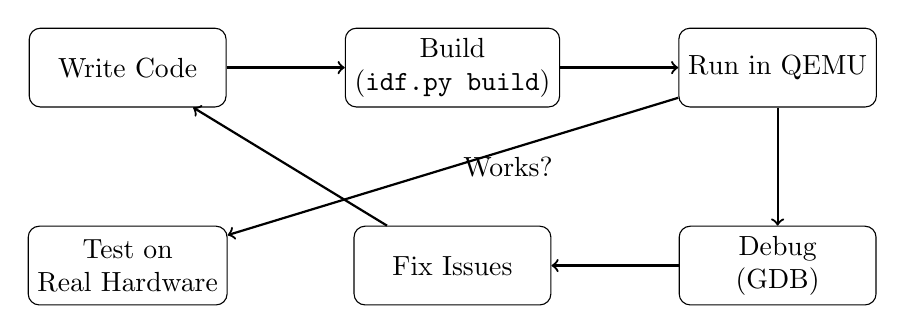
\begin{tikzpicture}[
        node distance=1.5cm,
        box/.style={rectangle, draw, rounded corners, minimum width=2.5cm, minimum height=1cm, align=center},
        arrow/.style={->, thick}
    ]
        \node[box] (write) {Write Code};
        \node[box, right=of write] (build) {Build\\(\texttt{idf.py build})};
        \node[box, right=of build] (run) {Run in QEMU};
        \node[box, below=of run] (debug) {Debug\\(GDB)};
        \node[box, below=of build] (fix) {Fix Issues};
        \node[box, below=of write] (test) {Test on\\Real Hardware};

        \draw[arrow] (write) -- (build);
        \draw[arrow] (build) -- (run);
        \draw[arrow] (run) -- (debug);
        \draw[arrow] (debug) -- (fix);
        \draw[arrow] (fix) -- (write);
        \draw[arrow] (run) -- node[right] {Works?} (test);
    \end{tikzpicture}
    \end{center}

    \vspace{0.3cm}
    \textbf{Advantages:}
    \begin{itemize}
        \item Fast iteration cycle
        \item No hardware needed for initial development
        \item Full debugging capabilities
    \end{itemize}
\end{frame}

%==============================================================================
% SECTION 7: Conclusion
%==============================================================================

\section{Conclusion}

% Slide 19: Course Approach
\begin{frame}{Our Course Approach}
    \textbf{We'll use a hybrid approach:}

    \vspace{0.3cm}
    \begin{enumerate}
        \item \textbf{Start with Arduino}
            \begin{itemize}
                \item Learn basics quickly
                \item Get comfortable with ESP32
                \item Build working projects fast
            \end{itemize}

        \vspace{0.3cm}
        \item \textbf{Transition to ESP-IDF}
            \begin{itemize}
                \item Understand what's ``under the hood''
                \item Learn professional development
                \item Build production-quality code
            \end{itemize}

        \vspace{0.3cm}
        \item \textbf{Use QEMU Throughout}
            \begin{itemize}
                \item Develop anywhere, anytime
                \item Consistent environment
                \item Better debugging
            \end{itemize}
    \end{enumerate}
\end{frame}

% Slide 20: Resources & Next Steps
\begin{frame}{Resources \& Next Steps}
    \textbf{Getting Started:}
    \begin{itemize}
        \item Clone the course Docker environment
        \item Run the example programs in \texttt{slides/examples/}
        \item Try modifying the blink rate!
    \end{itemize}

    \vspace{0.3cm}
    \textbf{Documentation:}
    \begin{itemize}
        \item Arduino ESP32: \texttt{docs.espressif.com/projects/arduino-esp32}
        \item ESP-IDF: \texttt{docs.espressif.com/projects/esp-idf}
        \item FreeRTOS: \texttt{freertos.org/Documentation}
    \end{itemize}

    \vspace{0.3cm}
    \textbf{Next Class:}
    \begin{itemize}
        \item Hands-on: Setting up your environment
        \item First project: Hello World on QEMU
    \end{itemize}

    \vspace{0.3cm}
    \begin{center}
        \textbf{Questions?}
    \end{center}
\end{frame}

\end{document}
